\documentclass[12pt]{article}

\usepackage{sbc-template}

\usepackage{graphicx,url}

\usepackage[brazil]{babel}   
\usepackage[utf8x]{inputenc}  

     
\sloppy

\title{Evoluindo os pesos de uma Rede Neural \\com Algoritmos Genéticos}

\author{Davi Azevedo Q. Santos\inst{1}, Derik Evangelista R. Silva\inst{1}, Aurora Trinidad R. Pozo\inst{1}}
  

\address{Departamento de Informática -- Universidade Federal do Paraná (UFPR)\\
  Caixa Postal 19081  -- 81531-980 -- Curitiba -- PR -- Brasil
  \email{\{daqsantos, dersilva, aurora\}@inf.ufpr.br}
}

\begin{document} 

\maketitle

\begin{abstract}
This paper compares the training of a Multi Layer Perceptron using two approaches: a pure Genetic Algoritthm and a hybrid one using backpropagation. Various combinations of genetic operators are applied to the problem of classification.The results should show that the best combination can meet or exceed the results obtained with the classic Backpropagation algorithm.
\end{abstract}
     
\begin{resumo} 
Este artigo compara o treinamento de um Multi Layer Perceptron usando duas abordagens: um Algoritmo 
genético puro e um híbrido usando backpropagation. Várias combinações de operadores genéticos são 
aplicadas para o problema de classificação. Os resultados devem mostrar que a melhor combinação consegue atingir ou ultrapassar os resultados obtidos com o algoritmo clássico de Back propagation.
\end{resumo}

\section{Introdução}

\par As Redes Neurais Aritificiais são uma das formas mais populares e efetivas para construção de sistemas de aprendizagem \cite{russel}, e são utilizadas nas mais diversas áreas, como, por exemplo, análise financeira \cite{bank}, medicina \cite{medic} e meteorologia \cite{forecast}. Representam uma flexível técnica heurística para reconhecimento de padrões \cite{duda}, além de possuirem a habilidade de realizar computação distribuída, tolerar entradas ruidosas e, é claro, aprender \cite{russel}.
\par A rede neural mais comumente utilizada é a Multi-layer Perceptron, na qual normalmente se utiliza o algoritmo \emph{back propagation} \cite{rumerhalt} para o treinamento dos pesos das conexões \cite{Liu}. Apesar da popularidade, o \emph{back propagation} tem algumas desvantagens. Por utilizar a gradiente descendente, a performance do treinamento está diretamente relacionada com a superfície de erro do problema, que pode conter mínimos locais, fazendo com que o gradiente descendente não encontre o mínimo global \cite{rumerhalt}.
\par Os algoritmos genéticos (AG) \cite{goldberg}, por sua vez, tem tido grande sucesso em problemas de busca e de otimização, principalmente em espaços de busca grandes, complexos e pouco conhecidos, onde os métodos de buscas convencionas (enumerativos, heurísticos, \dots) não são apropriados, oferecendo um método válido para pro\-ble\-mas que necessitam de uma busca eficiente e efetiva \cite{herrera}.
\par O objetivo deste trabalho é treinar uma rede neural artificial utilizando algorítmo genético. \cite{Liu} realiza o treinamento utilizando, além do AG, o \emph{back propagation} para refinar a solução encontrada. Já \cite{montana} utiliza um conjunto variado de operadores genéticos de mutação e cruzamento. Neste trabalho, implementaremos uma versão híbrida dos métodos de treinamentos propostos por \cite{Liu} e \cite{montana} e comparararemos os resultados do treinamento realizado com o AG puro contra o AG com \emph{back propagation}.
%\par \cite{Liu} realiza o treinamento de uma Rede Neural Artifical usando Algoritmos Genéticos (AG) para o problema de classificação de imagens. Além disso, o Backpropagation é utilizado como uma forma de busca local para refinar a solução encontrada pelo AG. \cite{montana}, por outro lado, utiliza um AG hibrido, onde é introduzido um operador de gradiente.

%O objetivo deste trabalho é treinar uma Rede Neural Artificial utilizando os mesmos operadores e comparar o resultado de um AG puro com um AG híbrido com backpropagation.

\par Este artigo está organizado da seguinte forma: no capítulo 2 são apresentados os conceitos de Redes Neurais Artificiais e Algoritmos Genéticos. No capítulo 3 são apresentados os detalhes de implementação, operadores genéticos e as bases de dados utilizados. O capítulo 4 expõe os resultados; e o capítulo 5, as conclusões.

\section{Metodologia} \label{sec:metodologia}

\subsection{Redes Neurais}
%\section{Redes Neurais}

\par Segundo \cite{kasabov} uma Rede Neural Artifical é um modelo computacional biologicamente inspirado no cérebro humano que consiste de elementos de processamento (neurônios) e conexões entre eles (pesos) que representam a memória do sistema. O primeiro modelo de neurônio artificial foi proposto por McCulloch e Pitts em 1943. 
\par Uma rede neural é definida por quatro parâmetros:

\begin{enumerate}
	\item Tipo de neurônio: determina como são tratados os valores de entradas e calculados de saída de um neurônio;
	\item Arquitetura conexionista: determina como os neurônios se conectam entre si;
	\item Algoritmo de aprendizado: determina como o conhecimento é armazenado na rede;
	\item Algoritmo de Recall: determina como o conhecimento da rede é recuperado.
\end{enumerate}

\par Os vários modelos de redes neurais artificais podem ser descritos em termos destes parâmetros. O modelo mais comum é o Multi Layer Perceptron (MLP), que consiste de uma arquitetura totalmente conectada entre as camadas, possui no mínimo três camadas (entrada, oculta e saída). Além disso, cada neurônio tem um entrada fixa (bias), e a função de ativação mais usada é a sigmóide.

\par Neste trabalho utilizaremos o MLP para o problema de classificação. Segundo \cite{kasabov} O problema de classificacão é associar um objeto a um grupo ou classe de objetos já existentes. 

\par O MLP tornou-se bastante utilizado com surgimento do algoritmo Backprogation como algoritmo de aprendizado. Contudo, neste trabalho, para realizar o treinamento da rede neural, será implementado duas abordagens: uma utilizado um Algoritmo Genético puro e a outra um Algoritmo Genético híbrido, o qual introduz a execução do backpropagation logo após a aplicação dos operadores de mutação. Todavia, por conta do custo, apenas um pequeno número de iterações do backprogation será utilizado.

\subsection{Algoritmos Genéticos}
%\section{Algoritmos Genéticos}

\par O Algoritmo Genético (AG), geralmente referenciado como \emph{algoritmos genéticos}, foi desenvolvido por John Holland na Universidade de Michigan, em 1975, em um dos livros mais famosos da área, \emph{Adaptation in Natural and Artificial Systems}, publicado pela editora \emph{University of Michigan Press} \cite{essentials:pop}.
\par Os AGs são algoritmos de busca heurística que imitam artificialmente o processo de evolução, da Teoria de Evolução das Espécies, de Darwin. São muito similares a outros algoritmos de busca local, como o Subida de Encosta (\textit{Hill-climbing}), diferindo apenas na quantidade de soluções mantidas a cada iteração e no processo de geração de novas soluções.
\par De acordo com \cite{montana}, os AGs necessitam de cinco componentes:
\begin{enumerate}
\item[C1] - Uma maneira de codificar uma solução em um indivíduo.
\item[C2] - Uma função de avaliação que retorna um índice de qualidade para cada individuo da população.
\item[C3] - Um procedimento de inicialização da população.
\item[C4] - Operadores que podem ser aplicados nos indivíduos pais no processo de reprodução, alterado a composição genética dos novos indivíduos gerados. Neste componente incluem-se os operadores de mutação, de cruzamento, seleção e outros específicos do domínio.
\item[C5] - Uma configuração de parâmetros do algoritmo, os operadores, etc.
\end{enumerate}
Com estes cinco componentes, ainda de acordo com \cite{montana}, o AG funciona seguindo os seguintes passos:
\begin{enumerate}
	\item A população é iniciada usando-se o procedimento C3. O resultado é um conjunto de indivíduos, de acordo com C1.
	\item Cada indivíduo é avaliado, usando a função definida em C2.
	\item A população se reproduz até que um critério de parada seja atingido. A reprodução é realizada seguindo-se os seguintes passos:
	 \begin{enumerate}
		\item Um ou mais indivíduis são escolhidos para a reprodução. A seleção é estocástica, mas os pais melhores avaliados são favorecidos na escolha. Os parametros em C5 podem influenciar neste processo de seleção.
		\item Os operadores de C4 são aplicados aos pais para geração dos filhos. Os parametros em C5 ajudam a determinar quais operadores serão usados.
		\item Os filhos são então avaliados e inseridos de volta na população. Em algumas versões de AG, toda a população é substituida. Em outras, apenas um subconjunto é substituido.		
	\end{enumerate}
\end{enumerate}

\par A cada iteração, os indivíduos melhor avaliados tem mais chances de serem escolhidos para reprodução, fazendo com que, em teoria, sejam gerados melhores indivíduos a cada geração. Ao término do algoritmo, senão a ótima, a tendência é ter-se uma solução muito próxima a ela.


\section{Implementação}\label{sec:imple}

\par A linguagem Java foi utilizada para implementar os algoritmos. A rede neural foi codificada como um vetor de números em ponto flutuante, também conhecido como \textit{real-coded} \cite{Liu}. A figura \ref{fig:nn} ilustra esse processo, que foi baseado em \cite{montana}. Desta forma, é possível determinar rapidamente quais são os pesos de entrada e saída de cada neurônio e assim facilitar a implementação dos o\-pe\-ra\-do\-res genéticos. O número de camadas da rede é fixo e consiste em uma camada de entrada, uma camada oculta e uma camada de saída. 

\par  As bases de dados utilizadas foram retiradas de \cite{frank}. Para o experimento foram utilizadas as seguintes bases:

\begin{enumerate}
	\item \textit{Breast Cancer Wisconsin (Original) Data Set}, doravante denominada \textit{Câncer};
	\item \textit{Pima Indians Diabetes Data Set};
	\item \textit{Glass Identification Data Set};
	\item Statlog (Heart) Data Set, doravante denominada \textit{Heart};
	\item \textit{Iris Data Set}.
\end{enumerate}

\par Na tabela \ref{tab:params}, temos o número de neurônios de cada camada para cada base de dados a ser testada.

\begin{table}[h]
	\center
	\begin{tabular}{|c|c|c|c|c|}
		\hline Base  & Atributos (Entradas) & Classes (Saídas) & Ocultos \\ 
		\hline Cancer & 9 & 2 & 5 \\ 
		\hline Pima Indians Diabetes & 8 & 2 & 10 \\ 
		\hline Glass Identification & 9 & 7 & 10 \\ 
		\hline Heart & 13 & 2 & 5 \\ 
		\hline Iris & 4 & 3 & 10 \\ 
		\hline 
	\end{tabular}
	\caption{Número de neurônios de cada camada}
	\label{tab:params}
\end{table} 

\begin{figure}[ht]
\centering
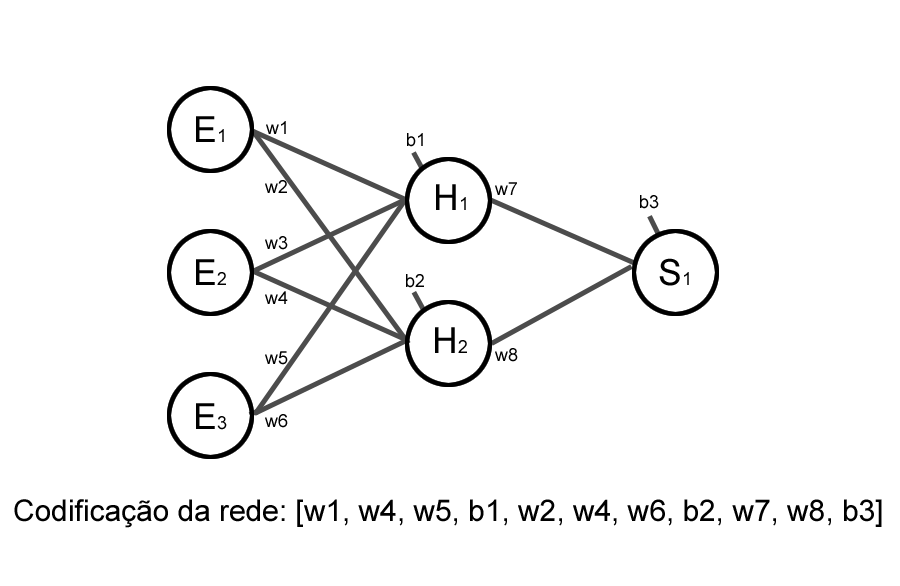
\includegraphics[width=80mm]{codificacao.png}
\caption{Codificacão da rede}
\label{fig:nn}
\end{figure}

\par O Algoritmo Genético foi implementado conforme \cite{essentials}. O \textit{fitness} de cada indivíduo é dado pelo Erro Quadrado Médio (EQM), ou seja, um indivíduo mais apto é aquele que possui o menor valor. O EQM é calculado de acordo com \cite{Liu}. 

\par A seguir temos operadores genéticos utilizados. Seus parâmetros, quando possivel, foram os mesmos das respectivas referências.

\begin{enumerate}
	\item Operadores de Mutação descritos em \cite{montana} e \cite{Liu} são:
	\begin{enumerate}
		\item Biased Mutate Weights: O valor de um gene pode ser substituído por um outro qualquer da distribuição de probabilidade inicial (distribuição normal com média 0 e desvio padrão 5).
		\item Unbiased Mutate Weights: Um valor da distribuição de probabilidade inicial é acrescido a um gene.
		\item Mutate Nodes: Este operador seleciona n neurônios das camadas oculta e de saída e adiciona um valor da distribuição de probabilidade inicial a cada peso de entrada dos neurônios. Nos nossos o valor de n foi 2.
		\item Mutate Weakest Nodes: Este operador seleciona o neurônio mais fraco (aquele que menos contribui para o saída da rede) e aplica uma mutação \textit{unbiased} ou \textit{biased} em cada peso do neurônio mais fraco.
		\item SinglePointRandom: Cada gene do cromossomo é substituído por um valor aleatório entre [-50, 50].
		\item NonUniform: implementado conforme \cite{Michalewicz}. Na nossa implementacão o parâmetro b é 4.
		
	\end{enumerate}

	\item Operadores de Crossover, segundo \cite{montana} e \cite{Liu}:
	\begin{enumerate}
		\item Crossover Weights: O valor gene de um indivíduo filho é escolhido pela seleção aleatória do mesmo gene de um dos pais.
		\item Crossover Nodes: Para cada neurônio de um dos pais escolhidos aleatoriamente os pesos associados são passados diretamente para o filho.
		\item Crossover Features: Para cada neurônio da rede do primeiro pai, o algoritmo reorganiza o segundo pai de forma que os neurônios que desempenham o mesmo papel (isto é, possum a mesma saída para uma determinada entrada) fiquem na posição, assim formando um pai intermediário. Depois disso é aplicado o operador Crossover-Nodes entre o primeiro pai e o pai intermediário.
		\item Line Recombination: A implementação foi um hibrido entre \cite{Liu} e \cite{essentials} onde o parâmetro é dado por uma distribuição normal com média 0 e desvio padrão 5.
	\end{enumerate}

\end{enumerate}

\par O operador de seleção utilizado, diferente de \cite{Liu} e \cite{montana}, foi o torneio. 


\par Além disso foi implementado, para efeitos de comparação, um AG híbrido com backpropagation. A implementacão foi confome \cite{freeman}. Contudo, diferente de \cite{Liu}, neste experimento são executadas cinco iterações do backpropagation logo após a aplicacão dos operadores de mutação, com a finalidade de refinar as soluções 

\par Os parâmetros utilizados para o Algoritmo Genético foram os seguintes:
\begin{enumerate}
	\item Tamanho da População: 50 e 100 indivíduos;
	\item Número de Gerações: 500;
	\item Tamanho do torneio: 2 e 4;
	\item Número de indivíduos da elite: 10;
	\item Probabilidade de Crossover: 100\%;
	\item Probabilidade de mutação: 10\%.
\end{enumerate}

\par Para a análise dos resultados foi utilizado a média da taxa de acerto das 10 execuções para cada combinação de parâmetros (população, tamanho do torneio, operador de mutação e crossover). O conjunto de dados foi separado de acordo com a tabela \ref{tab:db}.

\begin{table}
\center
\begin{tabular}{|c|c|c|c|}
\hline Base & Treinamento & Teste  & Total \\ 
\hline Cancer & 525 & 174 & 699 \\ 
\hline Pima Indians Diabetes & 510 & 258 & 768 \\ 
\hline Glass Identification & 164 & 50 & 214 \\ 
\hline Heart & 200 & 70 & 270 \\ 
\hline Iris & 110 & 40 & 150 \\ 
\hline 
\end{tabular} 
\caption{Separação dos conjuntos de dados}
\label{tab:db}
\end{table}


\section{Resultados obtidos}

Foram realizadas 10 execuções para cada combinação possível de:
\begin{enumerate}
\item Parâmetros do Algoritmo Genético (explicitados na seção \ref{sec:imple});
\item Operadores de mutação;
\item Operadores de cruzamento;
\end{enumerate}

Para os operadores de mutação e cruzamento, considerou-se também um operador extra, que seleciona aleatoriamente qualquer um dos operadores descritos. Nas figuras a seguir o eixo horizontal representa as gerações e o vertical o fitness médio de cada combinação de parâmetros.

\subsection{Influência dos parâmetros do AG}\label{res:ag}

De uma maneira geral, um tamanho de torneio maior mostrou ter um impacto positivo na média dos valores de fitness. Entretanto, a média piora em alguns casos ou, nos casos em que há melhora, ela é muito pequena, como podemos ver nas figuras \ref{fig:gla50.2} e \ref{fig:gla50.4}.

Analisando as figuras \ref{fig:dia50.4} e \ref{fig:dia100.4} podemos ver que um maior tamanho da população apresenta uma influência bem mais significativa que o tamanho do torneio em praticamente todas as execuções. Entretanto, ainda assim, a relação de consumo de recursos computacionais, associado ao maior tempo para execução e o ganho real de uma população maior pode não ser vantajoso.

\begin{figure}[htp]
\center
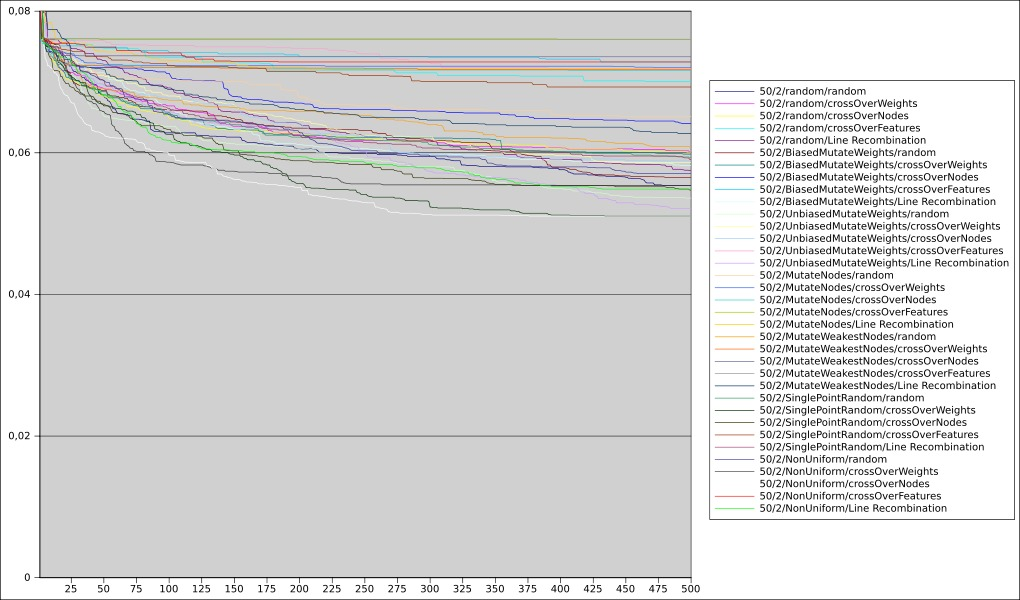
\includegraphics[scale=0.4, keepaspectratio]{glass_50_2.jpg} 
\caption{Fitness - Glass; População 50, torneio 2;}
\label{fig:gla50.2}
\end{figure}

\begin{figure}[hbp]
\center
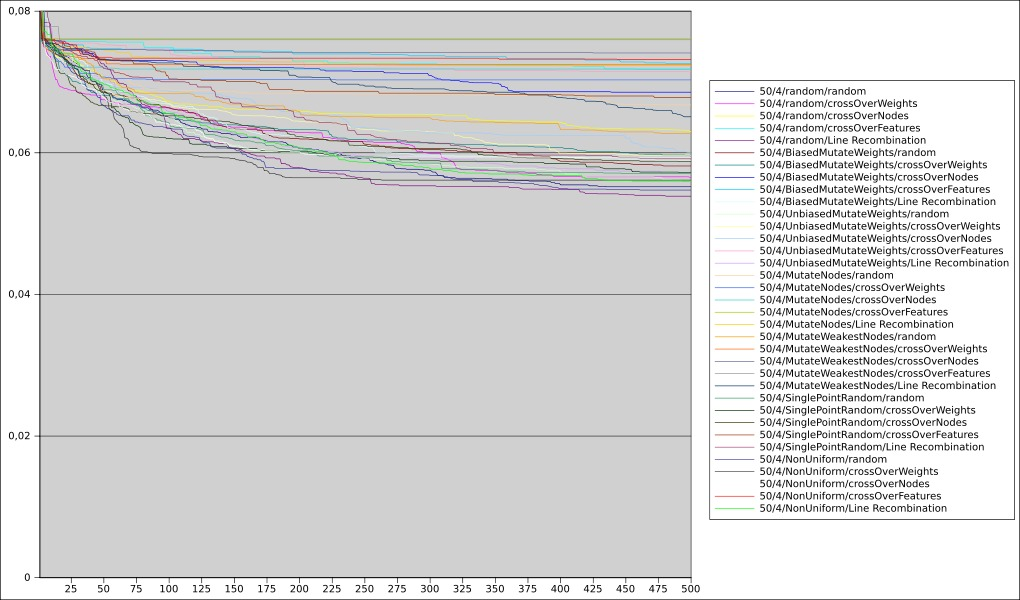
\includegraphics[scale=0.4, keepaspectratio]{glass_50_4.jpg} 
\caption{Fitness - Glass; População 50, torneio 4;}
\label{fig:gla50.4}
\end{figure}

\begin{figure}[htp]
\center
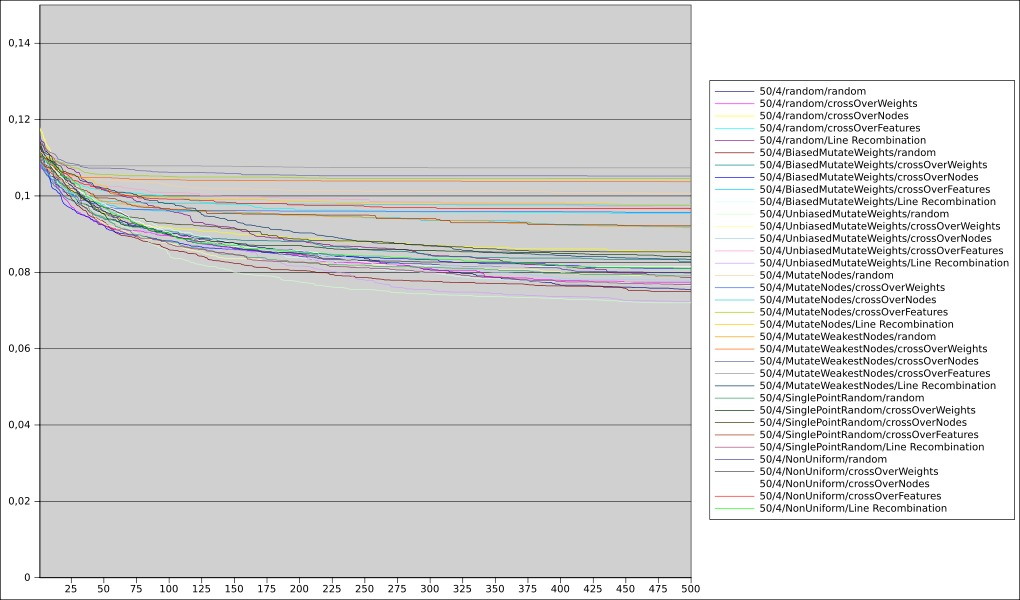
\includegraphics[scale=0.4, keepaspectratio]{dia_50_4.jpg} 
\caption{Fitness - Diabetes; População 50, torneio 4;}
\label{fig:dia50.4}
\end{figure}

\begin{figure}[hbp]
\center
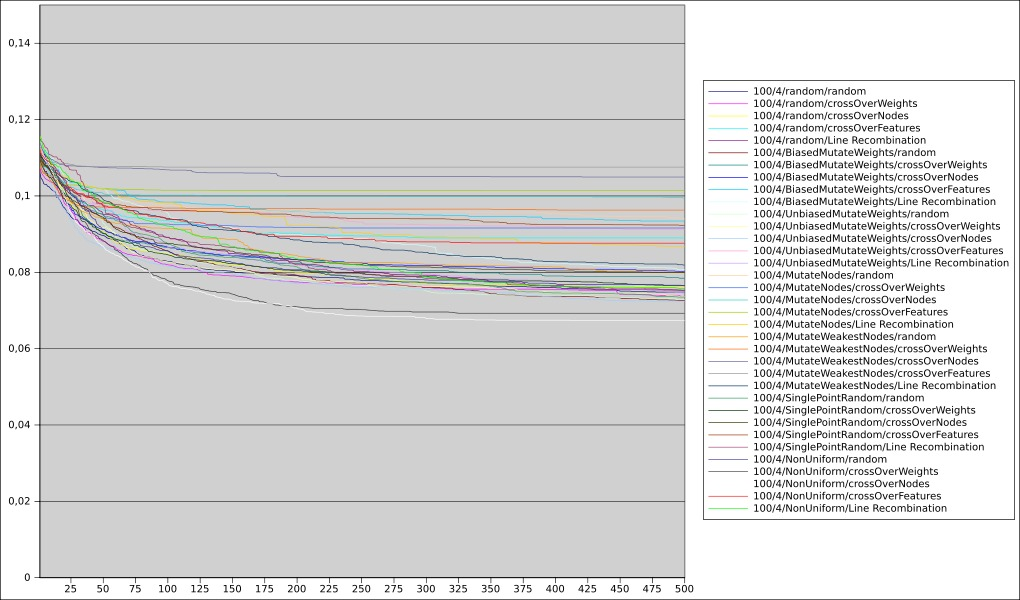
\includegraphics[scale=0.4, keepaspectratio]{dia_100_4.jpg} 
\caption{Fitness - Diabetes; População 100, torneio 4;}
\label{fig:dia100.4}
\end{figure}

\begin{figure}[htp]
\center
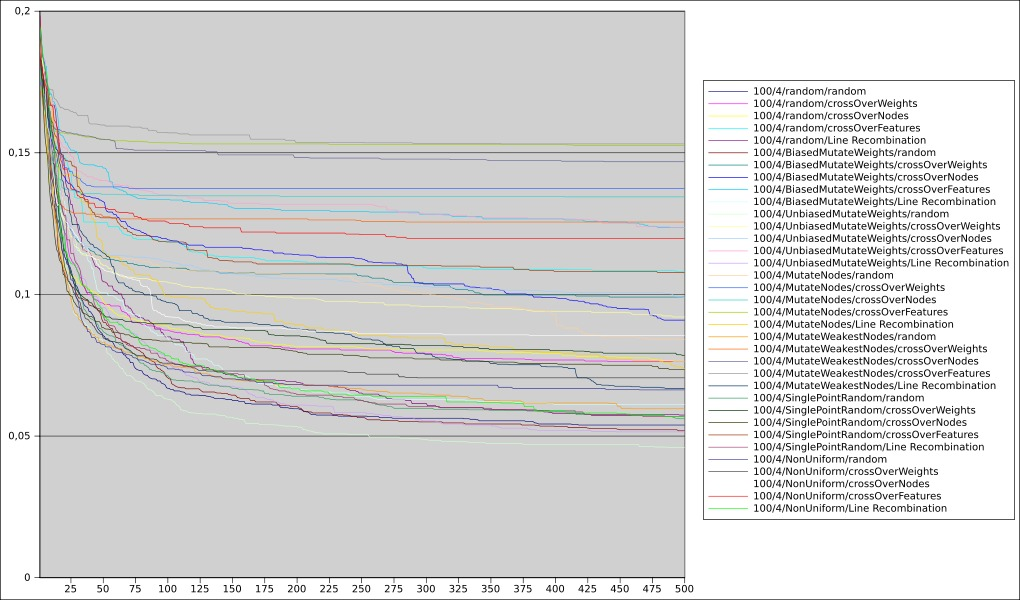
\includegraphics[scale=0.4, keepaspectratio]{hea_100_4.jpg} 
\caption{Fitness - Heart; População 100, torneio 4;}
\label{fig:hea100.4}
\end{figure}



\subsection{Influência dos Operadores Genéticos}

Diferentemente dos parâmetros em \ref{res:ag}, a escolha certa dos operadores genéticos tem um impacto muito grande. Podemos observar facilmente este impacto analisando a figura \ref{fig:hea100.4}: a diferença entre a pior combinação de operadores, que termina com a média de fitness um pouco maior que 0.15 e a melhor combinação, que termina com um valor de fitness menor que 0.05.

Também é interessante notar que em algumas casos, como o mostrado na figura \ref{fig:dia50.4}, muitas combinações de operadores mantem os valores de fitness muito próximos entre si e, como visto na figura \ref{fig:dia100.4}, há uma tendência a, em algum ponto, estabilizar, passando muitas gerações sem uma melhora sensível no valor. Estas características encontradas podem ser, em partes, remediadas aplicando-se, tal qual proposto por \cite{montana}, uma espécie de torneio com os operadores, dando preferência para aqueles que estão produzindo um maior impacto na rede.

\subsection{Taxas de Acerto}

Ao término das execuções, conseguimos analisar qual a taxa de acerto média da rede neural com seus pesos evoluidos através de um Algoritmo Genético.

Na tabelas \ref{tab:hitbest} e \ref{tab:hitbest2}, podemos visualizar as melhores taxas de acerto para o conjunto de testes com o AG puro e com o AG com back propagation, assim como qual combinação de parâmetros e operadores maximizou o acerto.  É interessante notar que o operador de cruzamento Line Recombination (dos cinco possíveis) foi que o conseguiu o melhor resultado na maioria das bases testadas. Já os operadores de mutação são mais heterogêneos. Podemos concluir, então, que o cruzamento tem um efeito maior na saída da rede que a mutação. Entretanto, se considerarmos que a mutação ocorre apenas em 10\% das vezes, ao passo que o cruzamento ocorre sempre, este comportamento é esperado.

Também podemos perceber que, em alguns casos, a rede se comportou melhor com uma população e torneio menores, embora na maior parte das execuções uma grande população e um maior tamanho de torneio tenham superado as outras combinações.

Ao compararmos as médias das duas abordagens (AG puro e AG híbrido), percebemos que, em geral, o back propagation melhorou o desempenho dos testes. Todavia, apenas na base Glass, o AG puro foi um pouco melhor. 

Na tabela \ref{tab:hitaim} temos os valores de acerto esperado para cada base. Comparando esta tabela com o resultado obtido, à exceção da base Câncer e Iris, o desempenho da rede foi bem abaixo do esperado, principalmente na bases Glass. Analisando as figura \ref{fig:gla50.4}, percebemos que o fitness para esta base converge rapidamente para um mínimo local e estaciona, não conseguindo sair deste mínimo. Por esse motivo, os valores encontrados para estas bases são relativamentes baixos. Outro ponto a ser notado, é que a base que possui o maior desvio padrão. Isso mostra que o AG tende a ficar preso em ótimos locais.

\begin{table}[h]
\center
\begin{tabular}{c|c|c|p{3cm}|p{3cm}|c|c|}
\cline{2-7}
&  \multicolumn{4}{|c|}{Parâmetros} & \multicolumn{2}{|c|}{Taxa de acerto} \\ \hline
\multicolumn{1}{|c|}{Base} & Pop & Tor & Mutação & Cruzamento & Média & Desvio padrão  \\ \hline
\multicolumn{1}{|c|}{Câncer} & 50 & 2 & Aleatório & Line Recombination & \textbf{0.961142} & 0.000908 \\ \hline
\multicolumn{1}{|c|}{Diabetes} & 100 & 2 & Unbiased Mutate Weights & Line Recombination & \textbf{0.663953} & 0.002083 \\ \hline
\multicolumn{1}{|c|}{Glass} & 100 & 4 & NonUniform & Aleatório & \textbf{0.414} & 0.029725 \\ \hline 
\multicolumn{1}{|c|}{Heart} & 100 & 4 & Single Point Random & Line Recombination & \textbf{0.784285} & 0.005421 \\ \hline
\multicolumn{1}{|c|}{Iris} & 100 & 4 & Unbiased Mutate Weights & Crossover Weights & \textbf{0.96} & 0.018973 \\ \hline
\end{tabular}
\caption{Melhores taxas de acerto para o AG puro}
\label{tab:hitbest}
\end{table}

\begin{table}[h]
\center
\begin{tabular}{c|c|c|p{3cm}|p{3cm}|c|c|}
\cline{2-7}
&  \multicolumn{4}{|c|}{Parâmetros} & \multicolumn{2}{|c|}{Taxa de acerto} \\ \hline
\multicolumn{1}{|c|}{Base} & Pop & Tor & Mutação & Cruzamento & Média & Desvio padrão  \\ \hline
\multicolumn{1}{|c|}{Câncer} & 50 & 4 & Biased Mutate Weights & Aleatório & \textbf{0.963218} & 0.00109 \\ \hline
\multicolumn{1}{|c|}{Diabetes} & 50 & 2 & Unbiased Mutate Weights & Line Recombination & \textbf{0.707751} & 0.017649 \\ \hline
\multicolumn{1}{|c|}{Glass} & 50 & 4 & Aleatório & Line Recombination & \textbf{0.306} & 0.020871 \\ \hline 
\multicolumn{1}{|c|}{Heart} & 50 & 4 & Single Point Random & Line Recombination & \textbf{0.798571} & 0.004969 \\ \hline
\multicolumn{1}{|c|}{Iris} & 50 & 4 & Unbiased Mutate Weights & Crossover Nodes & \textbf{0.9775} & 0.008696 \\ \hline
\end{tabular}
\caption{Melhores taxas de acerto para o AG com back propagation}
\label{tab:hitbest2}
\end{table}



\begin{table}[h!]
\center
\begin{tabular}{|c|c|c|}
\hline
Base & Taxa de acerto média & Desvio padrão\\ \hline
Câncer & 0.55 & 0.116563 \\ \hline
Diabetes & 0.46 & 0.195496 \\ \hline
Glass & 0.29 & 0.093893 \\ \hline
Heart & 0.52 & 0,079910 \\ \hline
Iris & 0.45 & 0.108857 \\ \hline
\end{tabular}
\caption{Taxas de acerto do back propagation}
\label{tab:hitaim}
\end{table}

\section{Considerações Finais}

Baseado na análise dos resultados obtidos, podemos notar que, apesar do algoritmo conseguir uma rápida queda nos valores de fitness em poucas gerações, o que aumenta as taxas de acerto da rede, a evolução dos pesos da rede sofre com o problema recorrente aos AGs, de otimização fina. Ao chegar em um certo valor de fitness, por mais que se alterem os códigos genéticos dos filhos, é muito difícil continuar a melhorar a rede, causando uma estagnação dos valores. É provavel que, mesmo que aumentemos o número de gerações, a melhora da rede seja ínfima. O mesmo acontece com o AG híbrido. Apesar de encontrar na maioria das vezes uma solução melhor o ganho geral é pequeno.

Para evitar isto, se faz necessário a criação de novos (e melhores) operadores genéticos, que consigam impactar a rede de forma que os pesos continuem a evoluir. Além disso, desenvolver um mecanismo de evolução dos operadores, conforme descrito por \cite{montana}, de forma que os operadores sejam escolhidos de acordo com o impacto que este teve anteriormente na rede, pode melhorar ainda mais a evolução dos pesos. Isto pode ser feito em trabalhos futuros.

\bibliographystyle{sbc}
\bibliography{sbc-template}

\end{document}
